%%%%%%%%%%%%%%%%%%%%%%%%%%%%%%%%%%%%%%%%%%%%%%%%%%%%%%%%%%%%%%%%%%
%%%%%%%% ICML 2013 EXAMPLE LATEX SUBMISSION FILE %%%%%%%%%%%%%%%%%
%%%%%%%%%%%%%%%%%%%%%%%%%%%%%%%%%%%%%%%%%%%%%%%%%%%%%%%%%%%%%%%%%%

% Use the following line _only_ if you're still using LaTeX 2.09.
%\documentstyle[icml2013,epsf,natbib]{article}
% If you rely on Latex2e packages, like most moden people use this:
\documentclass{article}

% For figures
\usepackage{graphicx} % more modern
%\usepackage{epsfig} % less modern
\usepackage{subfigure} 

% For citations
\usepackage{natbib}

% For algorithms
\usepackage{algorithm}
\usepackage{algorithmic}

\usepackage{scrextend}
\usepackage{tikz,pgfplots}

% As of 2011, we use the hyperref package to produce hyperlinks in the
% resulting PDF.  If this breaks your system, please commend out the
% following usepackage line and replace \usepackage{icml2013} with
% \usepackage[nohyperref]{icml2013} above.
\usepackage{hyperref}

% Packages hyperref and algorithmic misbehave sometimes.  We can fix
% this with the following command.
\newcommand{\theHalgorithm}{\arabic{algorithm}}

% Employ the following version of the ``usepackage'' statement for
% submitting the draft version of the paper for review.  This will set
% the note in the first column to ``Under review.  Do not distribute.''
\usepackage[accepted]{icml2013} 
% Employ this version of the ``usepackage'' statement after the paper has
% been accepted, when creating the final version.  This will set the
% note in the first column to ``Proceedings of the...''
% \usepackage[accepted]{icml2013}


% The \icmltitle you define below is probably too long as a header.
% Therefore, a short form for the running title is supplied here:
\icmltitlerunning{Using LSTMs to Model Programming Languages}

\begin{document} 

\twocolumn[
\icmltitle{Using LSTMs to Model Programming Languages}

% It is OKAY to include author information, even for blind
% submissions: the style file will automatically remove it for you
% unless you've provided the [accepted] option to the icml2013
% package.
\icmlauthor{Brendon Boldt}{brendon.boldt@gmail.com}
\icmladdress{Marist College,
            3399 North Rd. Poughkeepsie, New York 12601}

% You may provide any keywords that you 
% find helpful for describing your paper; these are used to populate 
% the "keywords" metadata in the PDF but will not be shown in the document
\icmlkeywords{boring formatting information, machine learning, ICML}

\vskip 0.3in
]

\begin{abstract} 
Recurrent neural networks (RNNs), specifically long-short term memory 
networks (LSTM) are particularly good at performing next word prediction 
on natural languages. This research 
investigates the ability for these same LSTMs to perform next “word” 
prediction on programming languages, namely the Java programming 
language. In order to be fed into the LSTM, Java source code had to 
undergo a transformation which preserved the logical structure of the 
source code and removed from the code various specificities such as 
variable names and literal values. A standard English corpora and four 
separate Java repositories were then tested with a standard LSTM. 
Results suggest that LSTM used can more effectively model the Java code 
than it can English. These findings could be useful in areas such as 
code prediction in IDEs or in automated code generation.
\end{abstract} 

\section{Introduction}
\label{submission}

Machine learning techniques of language modelling are often applied
to natural languages, but many of the techniques used to model
natural languages can be applicable to programming languages as well.
One such an application of a language model is next-word prediction
which can prove very useful for tasks from auto-completion to anomaly
detection. There has been research into programming language models
which use Bayesian statistical inference ($n$-gram models)
to perform next-word prediction \cite{Allamanis}.
Yet some of the most successful natural language models have been
built using recurrent neural networks (RNNs); their ability to
remember data over long sequences makes them particularly apt for
word prediction.

Specifically, long-short term memory (LSTM) RNNs have further improved
the basic RNN model by increasing the ability of an RNN to remember
data over a longer sequence of input without the signal decaying
quickly \cite{LSTMArticle}. LSTMs are a sequence-to-word language
model which means given a sequence of words (e.g., words in the
beginning of a sentence), the model will produce a probability
distribution describing what the next word in the sequence is.
The equation below illustrates the basic structure of a
sequence-to-word language model where $L$ is the language model,
$w_i$ is the $i$th word in the sequence, and $W_{n+1}$ is a vector
describing the probability distribution describing which word $w_{n+1}$
is.

\begin{equation}
\label{seqtoword}
    L(w_1, w_2, w_3, \dots, w_n) = W_{n+1}
\end{equation}

We are specifically investigating next-statement prediction in method
bodies. While other parts of Java source code (e.g., class fields,
import statements) do have semantic significance, method bodies make up
the functional aspect of source code\footnote{
Functional insofar as method bodies describe that actual
behavior of the program.} and most resemble natural language sentences.
Just as individual semantic tokens (words) comprise natural language
sentences, statements, which can be thought of as semantic tokens,
comprise method bodies. Furthermore, the semantics of individual natural
language words coalesce to form the semantics of sentence just as the
semantics of the statement in a method body form the semantics of the
method as a whole. By this analogy, language modelling techniques which
operate on sentences comprised of words could apply similarly to method
bodies comprised of statements.

%~%~% Also \subsubsection{}

%should be given.  See Section~\ref{final author} for details of how to

\section{Tokenizing Java Source Code}

We are specifically looking at predicting the syntactic structure  of next 
statement in within Java source code method bodies. The syntactic structure 
of a complete piece of source code is typically represented in an abstract 
syntax tree (AST) where each node of the tree represents a distinct 
syntactic element (e.g., statement, boolean operator, literal integer). 
Method bodies are, in particular, comprised of statements which, more or 
less, represent a self-contained action. Each of these statements is the 
root of its own sub-AST which represents the syntactic structure of only 
that statement. For this reason, the statements are the smallest 
independent, semantically meaningful unit of a method body and are suitable 
to be tokenized for input into the RNN.

Nguyen et al. \cite{Nguyen} present a model for syntactic statement prediction 
called ASTLan which uses Bayesian statistical inference to interpret and 
predict statements in the form of sequential statement ASTs. While Bayesian 
statistical inference can be applied to statements directly in their AST 
form, RNNs operate on independent tokens such as English words. Thus, it is 
necessary that statement ASTs be flattened into a tokenized form in order to 
be used in an RNN language model.

\subsection{Statement-Level AST Tokenization}

The RNN model described in \citet{LSTMArticle} specifically uses space-delimited 
text strings, hence, when the statement ASTs are tokenized, they 
must be represented as space-delimited text strings.

To show the tokenization of Java source, take the following Java statement:

\begin{verbatim}
    int x = obj.getInt();
\end{verbatim}

The corresponding AST, as given by the Eclipse AST parser, appears in Figure \ref{ast-figure}.

\begin{figure}[ht]
\vskip 0.2in
\begin{center}
\centerline{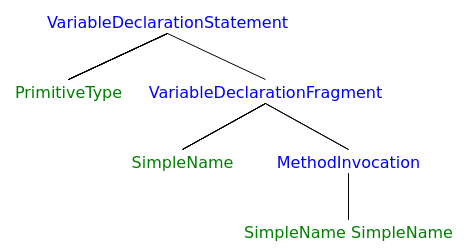
\includegraphics[width=\columnwidth]{ast.png}}
\caption{The abstract syntax tree (AST) representation of of the Java statement \texttt{int x = obj.getInt();}}
\label{ast-figure}
\end{center}
\vskip -0.2in
\end{figure} 

This statement, in turn, would be transformed into the following token.\footnote{
\texttt{VariableDeclarationStatement} is not included in the
tokenized version of the AST since the syntax is adequately represented
by starting with the root node's children.}

%~%~% Say why `VariableDeclarationStatement` does not appear

%\begin{addmargin}[0.5in]{0in}
\begin{verbatim}
    _PrimitiveType_VariableDeclarationFr
    agment(_SimpleName_MethodInvocation(_
    SimpleName_SimpleName)))

    _60(_39_59(_42_32(_42_42)))
\end{verbatim}
%\end{addmargin}

In the actual representation, the AST node names are replaced with integers IDs, but we 
have included the named version to demonstrate how it fits in with the visual AST. 
Individual AST nodes are separated by underscores (``\texttt{\_}'') and parentheses are 
used to denote a parent-child relationship so that the tree structure of the  statement 
is preserved. In fact, it is possible  to recreate the syntax of the original source 
code from the the tokens; thus, this  tokenization is lossless in terms of 
\textit{syntactical} information  yet lossy in other areas (variable and function names 
and the like are omitted to make the model more  general). 


\subsection{Method-Level Tokenization}

Now we can look at an entire method

%\begin{addmargin}[0.5in]{0in}
\begin{verbatim}
    int foo() {
        int x = obj.getInt();
        if (x > 0) {
            x = x + 5;
        }
        return x;
    }
\end{verbatim}
%\end{addmargin}

Each statement in the method body is tokenized just as the single statement 
was above where the tokens are space delimited. Braces, while not 
statements, are included (denoted by ``\texttt\{'' and
``\texttt\}''  to retain the semantic structure of the method body. 
Note that the return type and parameters are included as the first 
token with a leading ``\texttt('' to denote that it is a method
signature (no other statement tokens begin with an open paren).
%Just as before, the named and the numbered  version are displayed for clarity.

%\begin{addmargin}[0.5in]{0in}
\begin{verbatim}
    (_39_42 { _60(_39_59(_42_32(_42_42)))
     _25(_27(_42_34) { _21(_7(_42_27(_42_
     34))) } _41(_42) } 
\end{verbatim}
%\end{addmargin}

%~%~% I will only include these data sets if I have time.
\iffalse
In addition to representing the only the syntactic structure of the AST, tokens 
can also be generated to include the following information: the name of the 
type specified (e.g., in the case of PrimitiveType or ReferenceType), the 
specific operator (e.g., in the case of InfixExpression, PrefixExpression, 
etc.), and certain frequently occurring constants (e.g., \texttt 0,
\texttt 1, \texttt{true}, \texttt{false}, 
et&c.).

%\begin{addmargin}[0.5in]{0in}
\begin{verbatim}
    (_39:int_42 { _60(_39:int_59(_42_32(_
    42_42))) _25(_27:>(_42_34:0) { _21(_7
    (_42_27:+(_42_34))) } _41(_42) }
\end{verbatim}
%\end{addmargin}
\fi

The space-delimited sequence of these tokens forms a ``sentence'' which  
directly  correlates to the body of a single Java method. These individual  
tokens will then comprise the vocabulary which the LSTM network uses to train 
and make predictions with.

\subsection{English and Java Source Corpora Used}

Similarly to \citet{LSTMArticle}, We are using the Penn Treebank (PTB) for the
English language corpus as it provides an effective, general sample of the English
language. %~%~% Back this up?
For the Java programming languages, four different corpora were built from
the source code of projects (one project is built into one corpus). The
Java Development Kit (JDK), Google Guava, ElasticSearch, and Spring Framework.
The JDK is a good reference for Java since it is largest implementation
of the Java language; the other three projects were selected based on their
high popularity on GitHub in addition to the fact they are
Java-based projects.

It is important to note that the
Penn Treebank does not contain any punctuation while the tokenized
Java source contains ``punctuation'' only in the form of statement
body-delimiting curly braces (``\texttt\{'' and ``\texttt\}'')
since these are integral to the semantic structure of source code.

%~%~% Do I need to talk about this table at all?

\begin{table}[t]
    \caption{Total size of each corpora measured in words. The approximate
    split between training, validation, and test data is $80\%$, $10\%$,
    and $10\%$ respectively.}
    \label{size-table}
    \vskip 0.15in
    \begin{center}
    %\begin{small}
    \begin{tabular}{lr}
    \hline
    Corpus & \multicolumn{1}{c}{Size} \\
    \hline
    \abovespace
    PTB                 & $1085779$ \\
    JDK                 & $303560$ \\
    Guava               & $259686$ \\
    ElasticSearch       & $561697$ \\
    \belowspace
    Spring Framework    & $526968$ \\
    \hline
    \end{tabular}
    %\end{small}
    \end{center}
    \vskip -0.1in
\end{table}


\subsection{Vocabulary Comparison}

In addition to preserving the logical structure of the source code when
tokenizing it, another goal of the specific method of tokenization was to
produce a vocabulary with a frequency distribution similar to that of
English (compared against the English corpora used, that is). If the same
Java statement tokens appear too frequently, the tokenization might be
generalizing the Java source too much such that it loses the underlying
semantics. If the statement tokens, instead, all have a very low frequency
it would be difficult to effectively perform inference on the sequence of 
tokens within the allotted vocabulary size.

In all of the Java corpora,, the left and right curly braces comprise $~35\%$
of the total tokens present. This a disproportionately high number in
comparison to the rest of the tokens, but removing them from the frequency
distribution, since they classify as punctuation, gives a more accurate
representation of the vocabularies. The adjusted frequency distribution
shown in Figure \ref{english-frequency} compares the Penn Treebank to the
Java Development Kit source code. The rate of occurrence for the highest
ranked words is significantly higher in the JDK than in the PTB, but
the frequency distributions track closely together beyond the fifth-ranked
words. 

\begin{figure}
\begin{tikzpicture}
	\begin{axis}[
	    %height=5cm,
	    %width=8cm,
		xlabel=Word Rank,
		ylabel=Frequency,
		xmin=0,
		xmax=30]
		\addlegendentry{PTB}
		\addplot [dashed] table [
	    	x=rank,
		    y=PTB,
		    mark=none,
		    col sep=tab] {freq.dat};
		\addlegendentry{JDK}
		\addplot table [
	    	x=rank,
		    y=JDK,
		    mark=none,
		    col sep=tab] {freq.dat};
	\end{axis}
\end{tikzpicture} 
\caption{Comparison of English and Java word frequency distributions.
    The $y$-axis represents the total proportion of the word with a given
    rank (specified by the $x$-axis).}
\label{english-frequency}
\end{figure}
 
Adjusting the four Java corpora in the same way (removing the left and right
curly braces) yields similar frequency distributions across all word ranks
(see Figure \ref{java-frequency}).
 
\begin{figure}
\begin{tikzpicture}
	\begin{axis}[
		xlabel=Word Rank,
		ylabel=Frequency,
		xmin=0,
		xmax=30]
		\addlegendentry{JDK}
		\addplot table [
	    	x=rank,
		    y=JDK,
		    mark=none,
		    col sep=tab] {freq.dat};
		\addlegendentry{Guava}
		\addplot table [
	    	x=rank,
		    y=Guava,
		    mark=none,
		    col sep=tab] {freq.dat};
		\addlegendentry{ElasticSearch}
		\addplot table [
	    	x=rank,
		    y=ElasticSearch,
		    mark=none,
		    col sep=tab] {freq.dat};
		\addlegendentry{Spring Framework}
		\addplot table [
	    	x=rank,
		    y=SpringFramework,
		    mark=none,
		    col sep=tab] {freq.dat};
	\end{axis}
\end{tikzpicture} 
\caption{Comparison of Java corpora frequency distributions}
\label{java-frequency}
\end{figure}

\iffalse
    Another consideration when comparing the English and Java corpora are the
    prevalence of the metatokens \texttt{<eos>} denoting the end of a
    sentence and \texttt{<unk>} denoting a token not contained in the vocabulary.
\fi


%~%~% Should I use the adjusted metrics here?
\begin{table}[t]
    \caption{Proportion and rank of the metatoken%s \texttt{<eos>} and
    \texttt{<unk>}. Proportions and ranks are from the adjusted Java corpora
    with the left and right curly braces removed.}
    \label{sample-table}
    \vskip 0.15in
    \begin{center}
    %\begin{small}
    %\begin{tabular}{lcccc}
    \begin{tabular}{lcc}
    \hline
    \abovespace\belowspace
         %& \multicolumn{2}{c}{\texttt{<eos>}} &
                %\multicolumn{2}{c}{\texttt{<unk>}} \\
        %Corpus & Prop. & Rk. & Prop. & Rk. \\
        %\hline
        %\abovespace
        %PTB                 & $0.0453$ & $3$ & $0.0484$ & $2$ \\
        %JDK                 & $0.2664$ & $1$ & $0.0724$ & $2$ \\
        %Guava               & $0.3245$ & $1$ & $0.0476$ & $5$ \\
        %ElasticSearch       & $0.2641$ & $1$ & $0.1618$ & $2$ \\
        %\belowspace
        %Spring Framework    & $0.3203$ & $1$ & $0.0873$ & $2$  \\
    Corpus & Proportion & Rank\\
    \hline
    \abovespace
    PTB                 & $0.0484$ & $2$ \\
    JDK                 & $0.0724$ & $2$ \\
    Guava               & $0.0476$ & $5$ \\
    ElasticSearch       & $0.1618$ & $2$ \\
    \belowspace
    Spring Framework    & $0.0873$ & $2$  \\
    \hline
    \end{tabular}
    %\end{small}
    \end{center}
    \vskip -0.1in
\end{table}

Another consideration when comparing the English and Java corpora is the
prevalence of the metatoken \texttt{unk} which denotes a token not contained
in the language model's vocabulary.
Due to the nature of LSTMs, the vocabulary of the language model is finite;
hence, any word not contained in the vocabulary is considered unknown.
We specifically used a vocabulary size of $10,000$. A vocabulary size which
is too small will fail to represents enough words in the corpus; the result
is the LSTM seeing a high proportion of the \texttt{unk} metatoken. A
vocabulary which is too large increases the computation required during
training and inference.
The proportion of \texttt{<unk>} tokens in both the English and the Java
source data sets (save for ElasticSearch) are $<10\%$ which indicates that
the $10,000$ word vocabulary accounts for approximately $90\%$ of the corpus'
words by volume. It is important that the Java copora's \texttt{<unk>}
proportion is not significantly higher than that of the Penn Treebank since
that would suggest that $10,000$ is too small a vocabulary size to describe
the tokenized Java source code.

\iffalse
It is the case, though, that all of the Java copora show much higher
\texttt{<eos>}. This indicates that the sentences of the Java copora have
a lower average word count.
%~%~% Does this affect anything?
\fi

\section{Language Modelling}
\label{language-modelling}

%\subsection{LSTM Neural Network}

In order to make a good comparison between language modelling in English
and Java, a model with demonstrated success at modelling English was
chosen. The model selected was a long-short term memory (LSTM) neural
network, a type of recurrent neural network (RNN), as described in
\citet{LSTMArticle}. This particular LSTM uses regularization via 
dropout to act as a good language model for natural languages
such as English \cite{LSTMArticle}.
%when measuring word level perplexity 

%~%~% Talk about training size at all?

The LSTM's specific configuration was the same as the ``medium''
configuration described in \citet{LSTMArticle} with the exception
that the data was trained for $15$ epochs as the validation cost
suggested that the model was overfitting past $15$ epochs on the data
sets tested. Notably, this model contains two RNN layers with a vocabulary
size of $10,000$ words.

%~%~% Do I need to be more specific?

Each corpora was split into partitions such that $80\%$ was training data
and the remaining $20\%$ was split evenly between test and validation
data. Perplexity, the performance metric of the LSTM, is determined by the
ability of the LSTM to perform sequence-to-word prediction on the test
set of that corpus. Perplexity represents how well the prediction (in the
form a probability distribution) given by the LSTM matches the actual
word which comes next in the sentence. A low perplexity means that the
language model's predicted probability distribution matched closely the
actual probability distribution, that is, it was better able to predict
the next word.

%\subsection{Language Modelling Metric}

We chose word-level perplexity was chosen as the metric for comparing the
language models' performance on the given corpora since it provides
a good measurement of the models overall ability to predict words
in the given corpus. Perplexity for a given model is calculated
by exponentiatiting (base $e$) the opposite of the mean
cross-entropy across all words in the test set.

\begin{equation}
\label{perplexity}
    P(L) = \exp\left(\frac{1}{N}\sum^{N}_{i=1} H(L,w_i)\right)
\end{equation}

Where $N$ is the test data set size, $L$ is language model, $w_i$
is the $i$th word in the test set, and $H(L, w)$ is the natural log
cross-entropy from $w$ to the prediction given by $L(w)$. A lower perplexity represents a language model with better prediction
performance. The cross-entropy is calculated by summing the 
product of the probability of that word appearing ($1$ for the
correct word and $0$ for all other incorrect words) and the
natural log of output value of LSTM's softmax layer.

\begin{equation}
\label{cross-entropy}
    H(L,w) = \sum_{i=1}^V p(w) \ln L(w)
\end{equation}

Since the probability of all incorrect words is $0$, the sum
can be reduced to $1$ times the the natural log of the probability
of the correct word as given by the LSTM.

\begin{equation}
    H(L,w) = \ln L_w(w)
\end{equation}


%~%~% Should I measure the entropy of the corpora?

\section{Results}

\begin{table}[t]
    \caption{Perplexities given by Equation \ref{perplexity}.}
        %Entropy is the Shannon entropy calculated using
        %$\ln(P) / \ln(2)$.}
    \label{result-table}
    \vskip 0.15in
    \begin{center}
    %\begin{small}
    \begin{tabular}{lc}
    \hline
    \abovespace\belowspace
    Corpus & Perplexity \\%& Entropy \\
    \hline
    \abovespace
    PTB                 & $85.288$ \\%& $6.414$ \\
    JDK                 & $21.808$ \\%& $4.447$ \\
    Guava               & $18.678$ \\%& $4.223$ \\
    ElasticSearch       & $11.397$ \\%& $3.511$ \\
    \belowspace
    Spring Framework    & $11.318$ \\%& $3.501$ \\
    \hline
    \end{tabular}
    %\end{small}
    \end{center}
    \vskip -0.1in
\end{table}

The results of running the LSTM on the data sets is displayed in
Table \ref{result-table}. All four Java data sets showed a drastic reduction
in perplexity compared to the English data set. This suggests that the
LSTM was able to more accurately model the pre-processed Java source code
than it could English.

\section{Conclusion}

The pre-processed Java code represents a very general and cursory
representation of the original code as it does not include anything such
as variable names or variable types. Future research along these lines
could account for information such as variable types, literal values,
operator values, etc. Additionally, other machine learning methods like
a naive Bayesian classifier could be paired with the LSTM to predict
variable names as well as the syntactic structure of the next statement.
It would also be beneficial to compare the modelling of Java with other
programming languages or to train the model across multiple repositories
in one language.

% Note use of \abovespace and \belowspace to get reasonable spacing 
% above and below tabular lines. 


%articles , conference publications \cite{langley00}, book chapters \cite{Newell81}, books \cite{DudaHart2nd}, edited volumes \cite{MachineLearningI}, 

% In the unusual situation where you want a paper to appear in the
% references without citing it in the main text, use \nocite
%\nocite{langley00}

\bibliography{example_paper}
\bibliographystyle{icml2013}
%\bibliographystyle{ieeetr}

\end{document} 
              \end{document} 
\end{document}              \end{document} 
              \end{document} 
\end{document} 


% This document was modified from the file originally made available by
% Pat Langley and Andrea Danyluk for ICML-2K. This version was
% created by Lise Getoor and Tobias Scheffer, it was slightly modified  
% from the 2010 version by Thorsten Joachims & Johannes Fuernkranz, 
% slightly modified from the 2009 version by Kiri Wagstaff and 
% Sam Roweis's 2008 version, which is slightly modified from 
% Prasad Tadepalli's 2007 version which is a lightly 
% changed version of the previous year's version by Andrew Moore, 
% which was in turn edited from those of Kristian Kersting and 
% Codrina Lauth. Alex Smola contributed to the algorithmic style files.  

  \iffalse
    \begin{algorithm}[tb]
       \caption{Bubble Sort}
       \label{alg:example}
    \begin{algorithmic}
       \STATE {\bfseries Input:} data $x_i$, size $m$
       \REPEAT
       \STATE Initialize $noChange = true$.
       \FOR{$i=1$ {\bfseries to} $m-1$}
       \IF{$x_i > x_{i+1}$} 
       \STATE Swap $x_i$ and $x_{i+1}$
       \STATE $noChange = false$
       \ENDIF
       \ENDFOR
       \UNTIL{$noChange$ is $true$}
    \end{algorithmic}
    \end{algorithm}
\fi

 